\let\textcircled=\pgftextcircled
\chapter{Algorithms}
\renewcommand{\ttdefault}{pcr}
\lstset{
	basicstyle=\small\ttfamily,
	captionpos=t,
	numbers=left,
	tabsize=4,
	keywordstyle=\bfseries,
	breaklines=true,
	columns=fullflexible,
	numbersep=-8pt, 
	frame = shadowbox,
	morekeywords={BEGIN, END, DISPLAY, INPUT, IF, ENDIF, WHILE, DO, ELSE, THEN, OR, OPEN, RETURN, WRITE, NEXT, FOR, APPEND, CLOSE, PASS, AND, OUTPUT}
}

\section{Information Surrounding Blockchain Development}

This section will explain concepts that are fundamental to blockchain development and will give an insight into how all the different parts work together to create a functioning network. \\

The runtime of a blockchain is the business logic that defines its behaviour. In Substrate-based chains, the runtime is referred to as the "state transition function"; it is where Substrate developers define the storage items that are used to represent the blockchain's state as well as the functions that allow blockchain users to make changes to this state. Thus, the runtime can simply be thought of as the business logic of the chain. It defines what transactions are valid and invalid and determines how the chain's state changes in response to transactions.\\

The "outer node", everything other than the runtime, does not compile to WASM, only to native. The outer node is responsible for handling peer discovery, transaction pooling, block and transaction gossiping, consensus, and answering RPC calls from the outside world. While performing these tasks, the outer node sometimes needs to query the runtime for information or provide information to the runtime. A Runtime API facilitates this kind of communication between the outer node and the runtime. \\

An extrinsic is a piece of information that comes from outside the chain and is included in a block. Extrinsics fall into three categories: inherents, signed transactions, and unsigned transactions. A block in Substrate is composed of a header and an array of extrinsics. The header contains a block height, parent hash, extrinsics root, state root, and digest.  Extrinsics are bundled together into a block as a series to be executed as each is defined in the runtime. \\

Blockchains must agree on:

\begin{itemize}
	\item Some initial state, called "genesis", 
	\item A series of state transitions, each called a "block", and
	\item A final (current) state.
\end{itemize}

In decentralized systems, the nodes will see transactions in different orders, and thus they must use elaborate method to exclude transactions. As a further complication, blockchain networks strive to be fault tolerant, which means that they should continue to provide consistent data even if some participants are not following the rules. \\

Blockchain nodes use consensus engines to agree on the blockchain's state. It has some internal state, and state transition function that allows it to transition from its current state to a future state. In most runtimes there are states that have valid transitions to multiple future states, but a single transition must be selected. \\

Some nodes in a blockchain network are able to produce new blocks, a process known as authoring. This is decided by the consensus engine that is being used. For this permissoned blockchain, the consensus method that will be used is Aura (round-robin). Aura provides a slot-based block authoring mechanism where a known set of authorities take turns producing blocks. Further, a fork choice rule is an algorithm that takes a blockchain and selects the "best" chain, and thus the one that should be extended. The longest chain rule simply says that the best chain is the longest chain. \\

Users in any system want to know when their transactions are finalized, and blockchain is no different. In some traditional systems, finality happens when a receipt is handed over, or papers are signed. Using the block authoring schemes and fork choice rules described so far, transactions are never entirely finalized. There is always a chance that a longer (or heavier) chain will come along and revert your transaction. However, the more blocks are built on top of a particular block, the less likely it is to ever be reverted. In this way, block authoring along with a proper fork choice rule provides probabilistic finality. When deterministic finality is desired, a finality gadget can be added to the blockchain's logic. Members of a fixed authority set cast finality votes, and when enough votes have been cast for a certain block, the block is deemed final. In this system, this threshold is 2/3. Blocks that have been finalized by such a gadget cannot be reverted without external coordination such as a hard fork. The gadget that will be used is GRANDPA or GHOST-based Recursive Ancestor Deriving Prefix Agreement.
GRANDPA validators vote on chains, not blocks, i.e. they vote on a block that they consider "best" and their votes are applied transitively to all previous blocks. Once more than 2/3 of the GRANDPA authorities have voted for a particular block, it is considered final. A diagram of this process is below:\\

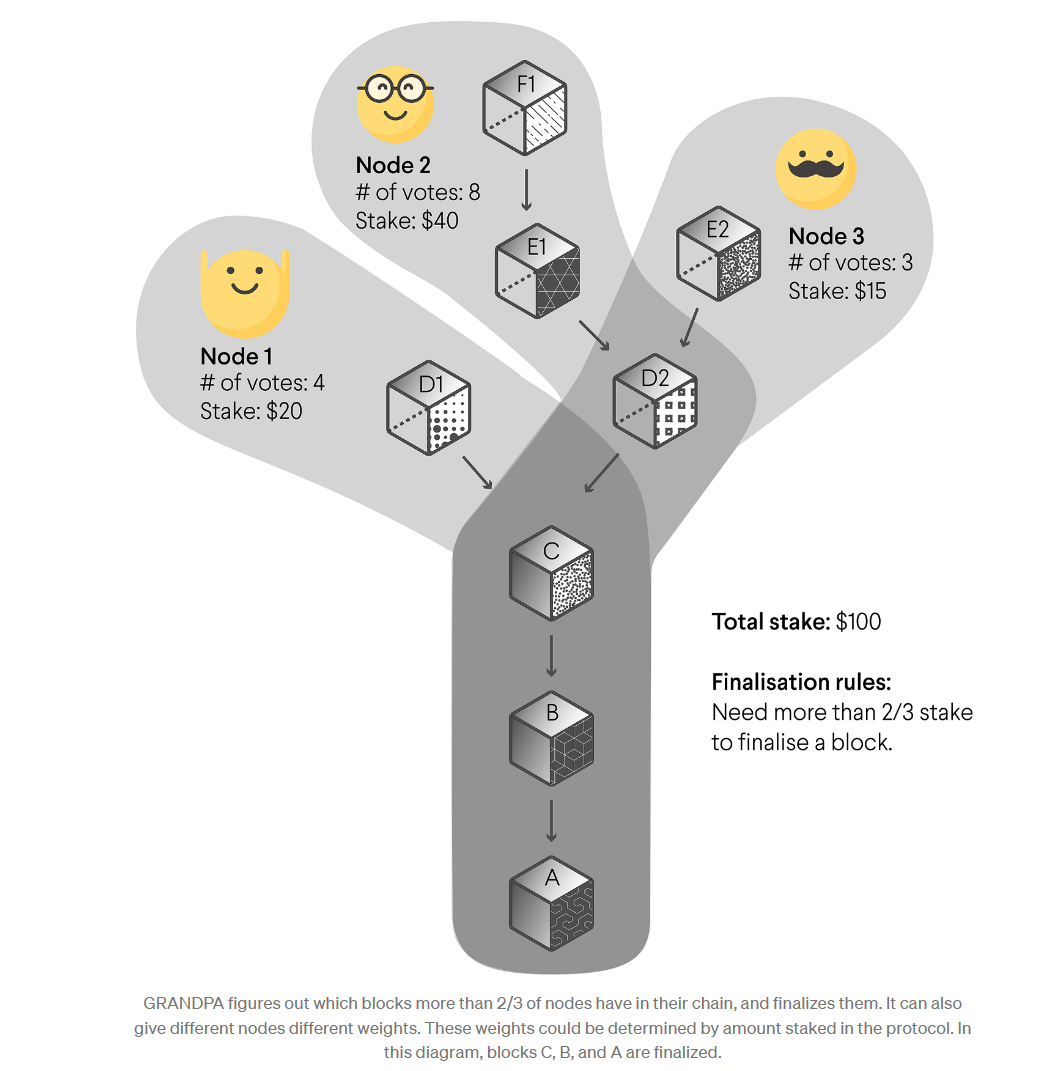
\includegraphics[width=\linewidth]{figures/finality.png} \\

Functions can be automated through smart contracts, in which lines of computer code use data from the blockchain to verify when contractual obligations have been met and payments can be issued. Smart contracts can be programmed to assess the status of a transaction and automatically take actions such as releasing a payment, recording ledger entries, and flagging exceptions in need of manual intervention. \\

Finally, a common architecture pattern for privacy-preserving is to only store a hash of the transaction data. For example, an invoice can be shared without exposing any details of the invoice. This allows companies to trace and exchange information with blockchain technology without exposing any data as the data are kept safely off-chain. \\

The core algorithms that will be used in the application are displayed below, written in the pseudo-code syntax. The program is split into two sections: the node that will be apart of the network, and the front-end that will be accessed by business's and clients after they have set up the node. For the purpose of the documentation each module will be represented by a single sub-routine, however, in production each module will have multiple files with many sub-routines for design organisation and efficiency. \\

\section{Algorithms - Node}
\subsection{Node Main Program}

\begin{lstlisting}[caption=Main Program, escapechar=\@]
	BEGIN MAINPROGRAM(node_key, port, ws_port, rpc_port, ed25519_key, sr25519_key, bootnodes)
		@\underline{services(node\_key, port, ws\_port, rpc\_port, ed25519\_key, }@ @\underline{sr25519\_key, bootnodes)}@ \\ This module starts a thread that spins up the network, client and extrinsic pool.
		@\underline{non\_fungible\_tokens(rpc\_port)}@ \\ Runtime "Pallet" that handles non-fungible token issuing and transference within the business blockchain. The RPC channel is the transmission line in that the interaction from the front end will go through.
		@\underline{fungible\_tokens()}@ \\ Runtime "Pallet" that handles fungible tokens and their minting, transference and architecture patterns.
		@\underline{runtime()}@ \\ This function/module handles all aspects of the runtime as described above.
	END MAINPROGRAM

\end{lstlisting}
\subsection{Runtime}
\begin{lstlisting}[caption=Runtime, escapechar=\@]
	BEGIN  @\underline{runtime(rpc\_port)}@
		runtime = new dataStructure with types BlockNumber, Signature, AccountId, Balance, Index, Hash

		let static const BLOCK_LENGTH = 5 * 1024 * 1024 \\ 5Mb
		let static const SLOT_DURATION = 6000 \\ This variable determines the average expected vlock time that is being targeted, this is 600 milliseconds or 6 seconds.

		@\underline{configure\_aura\_consensus()}@
		@\underline{configure\_grandpa\_finality()}@

		@\underline{configure\_transaction\_payments()}@
		@\underline{validate\_transactions()}@

		@\underline{configure\_node\_authorisation()}@ \\ This will enable nodes to be authorised while the blockchain is running, therefore the blockchain does not need to be stopped to allow people to join.

		FOR i=0 to rpc_port.extrinsics().length() DO
			@\underline{apply\_extrinsic(rpc\_port.extrinsics()[i])}@
		NEXT i

	END  @\underline{runtime()}@
\end{lstlisting}
\subsection{Non-fungible Tokens}
\begin{lstlisting}[caption=Non Fungible Tokens, escapechar=\@]
	BEGIN  @\underline{non\_fungible\_tokens(rpc\_port)}@
		let NFT = new dataStructure implementing config trait with fields price, owner and proof \\ Creates the NFT data structure that will represent each NFT item in the business blockchain.
		let Config = new Trait with types event, currency, MaxBytesInHash \\ The config trait that defines the parameters and types that the NFT pallet depends on.
		let NFTs = new StorageMap of NFT \\ Defines the storage structure in which NFT will be stored on the blockchain.
		let GenesisConfig = new empty NFTs Map \\ This defines the config for NFTs in the genesis block that all nodes must agree on, all nodes will start with an empty storage map for NFTs.
		
		IF rpc_port.recieve == "Create NFT" THEN \\rpc_port is the remote procedural call that is received from the web interface.
			@\underline{create\_nft(rpc\_port.user\_recieved(), rpc\_port.proof())}@
		ENDIF

		IF rpc_port.recieve == "Set Price" THEN
			@\underline{set\_price(rpc\_port.user\_recieved())}@
		ENDIF

		IF rpc_port.recieve == "Transfer" THEN
			@\underline{transfer(rpc\_port.user\_recieved(), rpc\_port.other())}@
		ENDIF

		IF rpc_port.recieve == "Buy NFT" THEN
			@\underline{buy\_nft(rpc\_port.user\_recieved(), rpc\_port.other())}@
		ENDIF
	END  @\underline{non\_fungible\_tokens()}@
\end{lstlisting}

\begin{lstlisting}[caption=Create NFT, escapechar=\@]
	BEGIN  @\underline{create\_nft(user, proof)}@ \\proof here a list of bytes which represent an image file, invoice, contract document that will be the foundation for the NFT.
		@\underline{ensure\_signed(user)?}@	
		let nft = new NFT using proof, user and block.
		let nft_id = @\underline{hash(nft)}@
		IF NFTs.contains(nft_id) == TRUE THEN
			OUTPUT("NFT already exists and cannot be replicated")
		ELSE
			NFTs.insert(nft_id)
		ENDIF
	END  @\underline{create\_nft()}@
\end{lstlisting}

\section{Algorithms - Front-end}

\subsection{Main Program}

\begin{lstlisting}[caption=Main Program, escapechar=\@]
	BEGIN  @\underline{frontend\_main(target\_url, api\_state, account)}@
		Connect to websocket using target_url
		IF api_state == "Error" THEN
			OUTPUT "API Error
		ENDIF

		IF api_state == "READY" THEN
			OUTPUT "Connecting to node"
			load_net(target\_url)
			load_acc(account)
		ENDIF

		@\underline{load\_frontend\_page(api)}@ \\ API is the data structure that represents the api that the front end is interacting with.
		@\underline{load\_nfts(api)}@
		@\underline{load\_fts(api)}@

	END  @\underline{frontend\_main()}@
			
\end{lstlisting}
\subsection{Display Non-fungible Tokens Module}

\begin{lstlisting}[caption=Load NFTs, escapechar=\@]
	BEGIN  @\underline{load\_nfts(api)}@
		let NFTs = @\underline{api\_query\_nfts()}@
		let fileReader = new fileReader \\ A new fileReader object which will enable the user to upload files on the web front end and for them to be read into a byte array.

		let elements = @\underline{load\_nft\_ui\_elements()}@

		let CreateNFT = new Button
		IF CreateNFT.pressed == TRUE THEN
			rpc.callable_function("create_nft(user, fileReader.file)")
		ENDIF

		IF element.transfer_button.pressed == TRUE THEN
			rpc.callable_function("transfer(user, to, nft_id)")
		ENDIF

		IF element.buy_nft.pressed == TRUE THEN
			rpc.callable_function("buy_nft(user, from, nft_id)")
		ENDIF

	END  @\underline{load\_nfts()}@
\end{lstlisting}


\vfill{}
